% This is samplepaper.tex, a sample chapter demonstrating the
% LLNCS macro package for Springer Computer Science proceedings;
% Version 2.21 of 2022/01/12
%
\documentclass[runningheads]{llncs}
%
\usepackage[T1]{fontenc}
% T1 fonts will be used to generate the final print and online PDFs,
% so please use T1 fonts in your manuscript whenever possible.
% Other font encondings may result in incorrect characters.
%
\usepackage[utf8]{inputenc}
\usepackage[english]{babel}
\usepackage{booktabs}
\usepackage{hyperref}
\usepackage{graphicx}
% Used for displaying a sample figure. If possible, figure files should
% be included in EPS format.
%
\usepackage[vlined,algoruled,linesnumbered]{algorithm2e}
\usepackage{amsmath,amssymb,nccmath,mathtools,stmaryrd}
\usepackage{tabularx}
\usepackage{multicol}
\usepackage{siunitx}
% If you use the hyperref package, please uncomment the following two lines
% to display URLs in blue roman font according to Springer's eBook style:
\usepackage{xcolor}
\renewcommand\UrlFont{\color{blue}\rmfamily}
\urlstyle{rm}
%
\begin{document}
%
\title{Masked Computation of the Floor Function and Its Application to the FALCON Signature}
%
\titlerunning{Masked Floor Function For FALCON}
% If the paper title is too long for the running head, you can set
% an abbreviated paper title here
%
\author{Justine Paillet\inst{1,3}\orcidID{0009-0009-6056-7766} \and
  Pierre-Augustin Berthet\inst{2,3}\orcidID{0009-0005-5065-2730} \and
C\'edric Tavernier\inst{3}\orcidID{0009-0007-5224-492X}}
%
\authorrunning{J Paillet et al.}
% First names are abbreviated in the running head.
% If there are more than two authors, 'et al.' is used.
%
\institute{
  Université Jean-Monnet, Saint-\'Etienne, France, \email{justine.paillet@univ-st-etienne.fr}
  \and
  Télécom Paris, Palaiseau, France, \email{berthet@telecom-paris.fr}
  \and
  Hensoldt SAS FRANCE, Plaisir, France, \email{<pierre-augustin.berthet,justine.paillet,cedric.tavernier>@hensoldt.net}
}
%
\maketitle              % typeset the header of the contribution
%
\begin{abstract}
With the ongoing standardization of new Post Quantum Cryptography (PQC) primitives by the National Institute of Standards and Technology (NIST), it is important to investigate the robustness of new designs to Side Channel Analysis (SCA). Amongst those future standards is Falcon, a lattice-based signature which relies of rational numbers. It thus requires an implementation using floating point arithmetic, which is harder to design well and secure. While recent work proposed a solution to mask the addition and the multiplication, some roadblocks remains, most noticeably how to protect the floor function. In this work we propose several methods to protect the computation of the floor function. We provide mathematical proofs of our methods as well as formal security proof in the probing model using the Non-Interference concepts. We also discuss their application to the FALCON Signature.

\keywords{Floor Function \and Floating-Point Arithmetic \and Post-Quantum Cryptography \and FALCON \and Side-Channel Analysis \and Masking}
\end{abstract}
%
%
%
\section{Notations}
\subsection{Diagram Legend}
\cite{10.1007/3-540-68697-5_9}
The following diagrams (\emph listofalldiagram figures) use the same legend:\begin{itemize}
    \item Probing sets are denoted by $P_i$ or $O$ and are colored in \textcolor{red}{red}.
    \item Simulation sets are denoted by $S_i^j$ and are colored in \textcolor{blue}{blue}.
    \item \emph{t-SNI} gadgets are colored in \textcolor{green}{green}.
    \item \emph{t-NI} gadgets are colored in \textcolor{black}{black}.
\end{itemize}
\section{Proofs}
\subsection{SetExZero}
\label{alg:setexzero}
\begin{figure}[!ht]
    \centering
    \includegraphics[width=7cm]{figure/SetExZero.pdf}
    \caption{Abstract diagram of Gadget \emph{SetExZero}}
    \label{fig:setexzero}
\end{figure}
\begin{lemma}\label{lem:setexzero}
    The gadget \emph{SetExZero} (Algorithm \ref{alg:setexzero}) is \emph{t-SNI} secure.    
\end{lemma}
\begin{proof}\label{proof:setexzero}
    We use an abstract diagram in Figure \ref{fig:setexzero} to demonstrate our proof. Let assume an adversary probes $t$ values, including the probing sets $P_i$ for $i\in\llbracket 1;5\rrbracket$. Let assume the simulation sets $S_i^j$ for some $j$ necessary to simulate the corresponding gadgets. \emph{t-SNI} security implies that if the size of all probing sets $P_i$ is $t_I\leq t$ and if the size of values required to simulate in each gadget is smaller than $t$, then the simulation sets linked to the input shares are not bigger than $t_I$.\newline
    \emph{SecAnd},\emph{SecOr} and \emph{A2B} being \emph{t-SNI} gagdets, we have the following:
    \begin{multicols}{2}
        \begin{itemize}
            \item $|S_1^1|,|S_1^2|\leq|P_1|$
            \item $|S_2^1|,|S_2^2|\leq|P_2|$
            \item $|S_3^1|,|S_3^2|\leq|P_3|$
            \item $|S_4|\leq|P_4|$
        \end{itemize}
    \end{multicols}
    Finally, \emph{-} being \emph{t-NI}, $|S_5|\leq|P_5|+|S_3^2|\leq|P_5|+|P_3|$. Based on the previous inequalities, one can check that no gadget requires more than $t_i$ values to be simulated. Finally, we can use at most $|S_4|\leq|P_4|$ shares of $ey$, $|S_3^1|\leq|P_3|$ shares of $b$ and $|S_5 \cup S_2^2| \leq |P_5| + |P_3| + |P_2|$ shares of $sy$ to simulate all the probed values, none being more than $t_I$.
\end{proof}

\subsection{SecFprUrshMod}
\label{alg:secfprurshmod}
\begin{figure}[!ht]
    \centering
    \includegraphics[width = 7cm]{figure/secfprurshmod.pdf}
    \caption{Abstract diagram for gadget \emph{SecFprUrshMod}}
    \label{fig:secfprurshmod}
\end{figure}
\begin{lemma}\label{lem:secfprurshmod}
    The gadget \emph{SecFprUrshMod} (Algorithm \ref{alg:secfprurshmod}) is \emph{t-SNI} secure.    
\end{lemma}
\begin{proof}
    We will make the same assumptions as in Proof \ref{proof:setexzero}. We rely on an abstract diagram of \emph{SecFprUrshMod} in Figure \ref{fig:secfprurshmod} to demonstrate our lemma. As the input shares are immediately fed into \emph{t-SNI} gadgets, we will check if the \emph{t-SNI} security holds for internal states of the algorithm. We have the following inequalities:
    \begin{multicols}{2}
        \begin{itemize}
            \item $|S_1^1|,|S_1^2|\leq|P_1|$
            \item $|S_2^1|,|S_2^2|\leq|P_2|$
            \item $|S_3|\leq|P_3| + |S_2^2| \leq |P_3| + |P_2|$
            \item $|S_4|\leq|P_4| + |S_3| + |S_1^2| \leq |P_4| + |P_3| + |P_2| + |P_1|$
            \item $|S_5^1|,|S_5^2| \leq |P_5|$
            \item $|S_6^1|,|S_6^2| \leq |P_6|$
        \end{itemize}
    \end{multicols}
    The number of values to simulate in each gadget is no more than $t_I$. This also applies to the input shares, with $|S_5^1| \leq |P_5|$ for $xi$, $|S_5^2 \cup S_6^1| \leq |P_5| + |P_6|$ for $ci$ and $|S_6^2| \leq |P_6|$ for $mi$.
\end{proof}

\subsection{RemoveDecimal}
\label{alg:removedecimal}
\begin{figure}[!ht]
    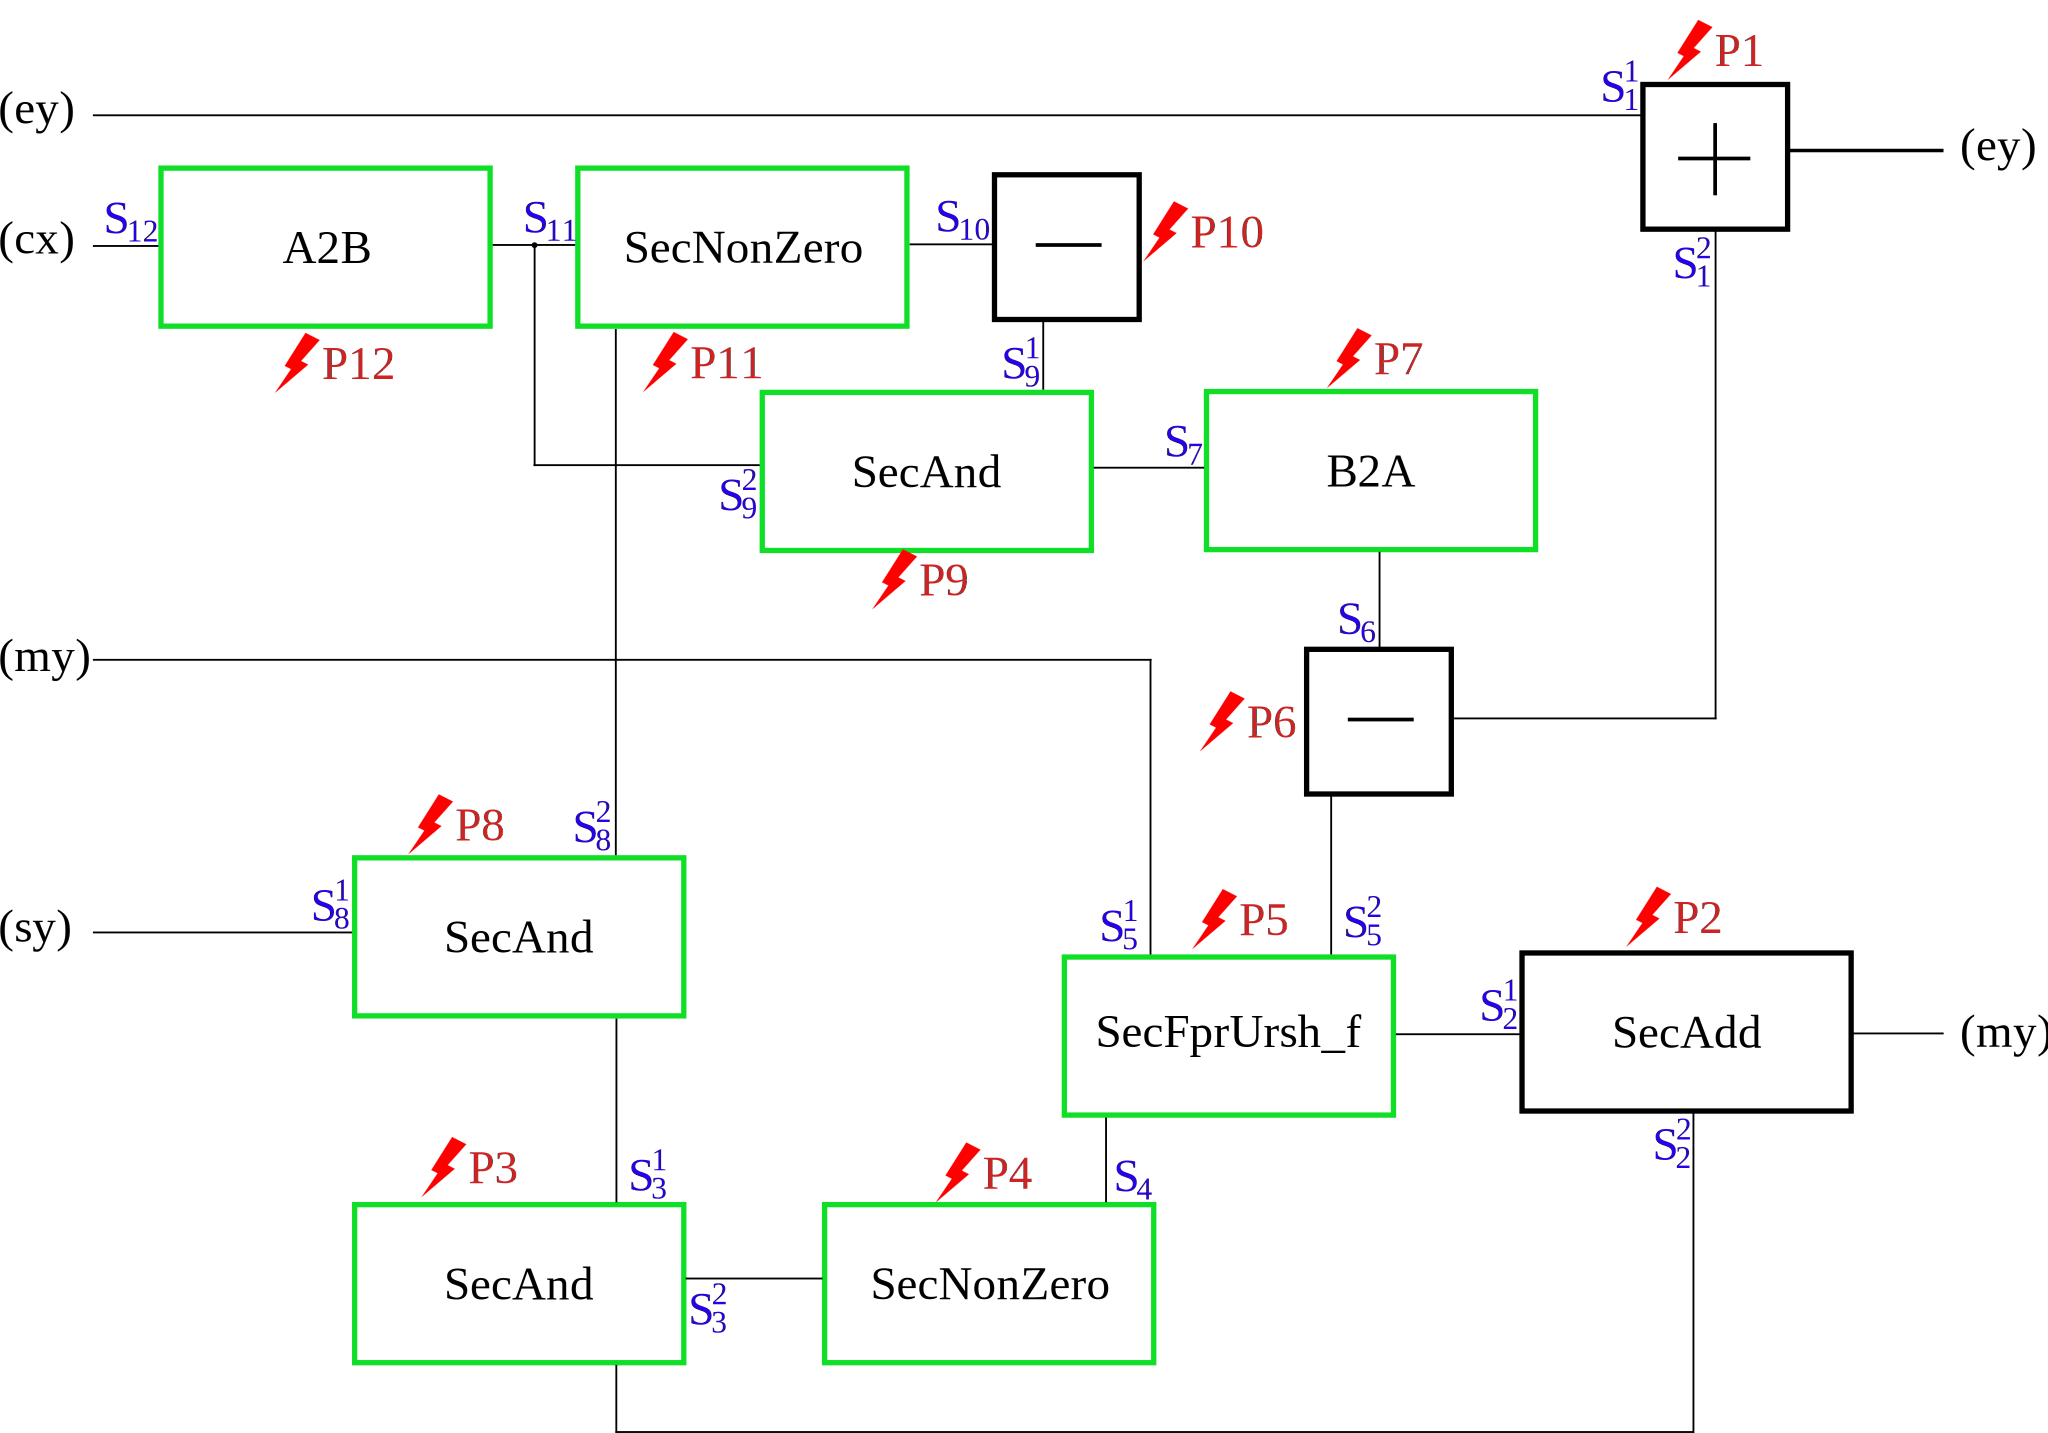
\includegraphics[width=7cm]{figure/RemoveDec.pdf}
    \caption{Abstract diagram for gadget \emph{RemoveDecimal}}
    \label{fig:removedecimal}
\end{figure}
\begin{lemma}\label{lem:removedecimal}
    The gadget \emph{RemoveDecimal} (Algorithm \ref{alg:removedecimal}) is \emph{t-SNI} secure.    
\end{lemma}
\begin{proof}
    We will make the same assumptions as in Proof \ref{proof:setexzero}. We use an abstract diagram of \emph{RemoveDecimal} in Figure \ref{fig:removedecimal} to demonstrate our lemma. We have the following inequaltities:
    \begin{multicols}{2}
        \begin{itemize}
            \item $|S_1^1|,|S_1^2|\leq|P_1| + |O_{ey}|$
            \item $|S_2^1|,|S_2^2|\leq|P_2| + |O_{my}|$
            \item $|S_3|\leq |P_3|$
            \item $|S_4|\leq|P_4|$
            \item $|S_5^1|,|S_5^2| \leq |P_5|$
            \item $|S_6| \leq |P_6| + |S_1^2| \leq |P_6| + |P_1| + |O_{ey}|$
            \item $|S_7|\leq|P_7|$
            \item $|S_8^1|,|S_8^2|\leq|P_8|$
            \item $|S_9^1|,|S_9^2| \leq|P_9|$
            \item $|S_10|\leq|P_10| + |S_9^1| \leq |P_10| + |P_9|$
            \item $|S_11| \leq |P_11|$
            \item $|S_12| \leq |P_12|$
            \item $|S_13| \leq |P_13|$
        \end{itemize}
    \end{multicols}
    
\end{proof}

\subsection{SecBaseInt}
\label{alg:secbaseint}
\begin{figure}[!ht]
    \includegraphics[width=7cm]{figure/secbaseint.pdf}
    \caption{Abstract diagram for gadget \emph{SecBaseInt}}
    \label{fig:secbaseint}
\end{figure}
\begin{lemma}\label{lem:secbaseint}
    The gadget \emph{SecBaseInt} (Algorithm \ref{alg:secbaseint}) is \emph{t-SNI} secure.    
\end{lemma}
\begin{proof}
    We will make the same assumptions as in Proof \ref{proof:setexzero}. We use an abstract diagram of \emph{SecBaseInt} in Figure \ref{fig:secbaseint} to demonstrate our lemma.
\end{proof}
%
% ---- Bibliography ----
%
% BibTeX users should specify bibliography style 'splncs04'.
% References will then be sorted and formatted in the correct style.
%
 \bibliographystyle{splncs04}
 \bibliography{falcon}

\end{document}
